\part{Rooms: geometry and design}

\chapter{Introduction}

\section{Blocks, sectors and clicks}

\textbf{Blocks, squares, sectors and clicks}: get used to these terms because you'll hear them frequently. The Tomb Editor is designed to work with a basic \emph{building block}, proportioned to Lara and her movements.
\par Levels are built by connecting a series of rooms comprised of walls and building blocks. The floor and ceiling of these rooms are sectioned into squares or sectors. The building blocks are created when you raise a square up from the floor or lower one down from the ceiling. Four mouse clicks up or down equals the width of these squares sections and creates a perfect cube \emph{Remember all those "blocks" Lara pushed and pulled around?!}
\par The building blocks are not limited to cubes and columns with flat tops. Corners of the surfaces can be pulled up or down to create angled slopes and \emph{organic} surfaces - great for creating rocky caves or sand dunes. \cite{trle_manual}

\section{Basic definitions}

Let's start with the default room: in the previous part, we've learnt that when we create a new level, TombIDE creates for us a level containing one room having size 18x18x3. Ok but.. 18x18x3 what?

It's time to introduce some formal definitions, forming a common dictionary.

\begin{remark}
    Property of a room is its \textbf{area}, measured in \emph{sectors} or \emph{squares}. This corresponds to the area of room's floor and room's ceiling, excluding walls.
\end{remark}

For our default room, its area is 18 squares. We can check it by alternatively counting squares in the Editor Windows, looking at the Sector Options or switching to the 2D mode in Tomb Editor.

Please note in the 3D view:
\begin{itemize}
    \item in the main editor window, floor and ceiling are represented in light blue color, while walls are represented in green;
    \item in the Sector Options panel, floor and ceiling are represented in light blue color, while walls are represented in grey.
\end{itemize}

\begin{remark}
    Given a room, the area of its floor is equal to the area of its ceiling.
\end{remark}

\begin{remark}
    Number of floor sectors is equal to number of ceiling sectors.
\end{remark}

Now, recall in mind a way to define position of objects in the three-dimensional space we live our life: we can rely on the cartesian coordinate system, where we use the three axes \( x, y, z\).
Up to now, we cared about \(x\) and \(y\). Let's introduce the way we can set \(z\) coordinate (height) and so, clicks:

\begin{remark}
    A \textbf{click} or full step is a linear transformation can be applied to a floor or a ceiling sector to increase or decrease its height.
\end{remark}

By using clicks, we can make a block.

\begin{remark}
    A \textbf{block} is the solid shape we can obtain by applying clicks to floor (raising) or ceiling (lowering).
\end{remark}

Finally, we reach the definition of the \emph{Tomb Raider cube}:
\begin{remark}
    A \textbf{Tomb Raider cube} is a cube-shaped block, where every edge is 4 clicks long.
\end{remark}

The definition of the Tomb Raider cube is useful because it's a simple way to remember Lara's sizes compared to her world and the real world.
Let's compare Lara's sizes and her movements with the cube, to better understand (\ref{fig:TIDELaraAndCube}).

\begin{remark}
    Lara's height is \emph{3 clicks}.
\end{remark}

\begin{remark}
    Assuming Lara's real height is 1.80m according to the original story \cite{wikiraider_LaraCroft}, a \emph{click} is 60cm and a \emph{Tomb Raider cube} is 2.40m high.
\end{remark}

\begin{figure}
    \centering
     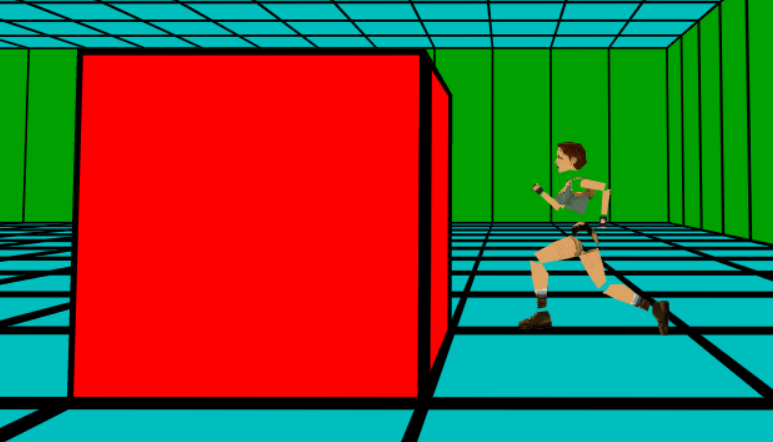
\includegraphics[width=1\textwidth]{screenshots/1010.png}
     \caption{Lara compared to the Tomb Raider cube.}
     \label{fig:TIDELaraAndCube} 
\end{figure}

In the next chapter we'll check together all the ways Tomb Editor provides us to model our room geometry. But before, we need to understand how we can move ourselves in the space.

\section{Tomb Editor 3D controls}

Open \emph{Test Level 1} we've created in the previous chapters. By default, the view is pointing to the north, to the center of the room, seen from above (45 degrees).
\par There are plenty of ways to move our view, basically looking at room and its contents from a different point in the space. Let's examine the available options.

\begin{itemize}
    \item \textbf{\keys{MW}}: by moving mouse wheel up and down, we can respectively increase or decrease the zoom. Geometrically, we are moving the camera along the vector perpendicular to its plan.
    \item \textbf{\keys{RMB} or \keys{\arrowkeyup \arrowkeydown \arrowkeyleft \arrowkeyright }}: by keeping the right mouse button down and moving the mouse, we can rotate the camera. Geometrically, we're moving the camera along the sphere centered to the point in front of our view. We can use arrow keys as well.
    \item \textbf{\keys{{MMB}}}: by keeping the scroll wheel button down and moving the mouse, we'll move the center of our view horizontally or vertically. Geometrically, we're moving the camera along its plan.
    \item \textbf{\path{View - Relocate camera} or \keys{ALT + z}}: mouse pointer will change to a cross. By \keys{LMB} we'll be able to set the new center of our view.
\end{itemize}

To \textbf{reset the camera position to its default} (useful in case you lost yourself), you can use \path{View - Reset camera position} or \keys{F6}.

\subsection{Fly mode}

There's another funny and useful way to move our point of view, through the \emph{fly mode}. Fly mode is activated by \path{View - Toggle fly mode} or \keys{SHIFT + z}.
\par Once activated, it's like being a fly! You can move your camera by combining:
\begin{itemize}
    \item mouse movement;
    \item \keys{WASDQE} keys;
    \item \keys{SHIFT} to go faster.
\end{itemize}

You can deactivate the fly mode anytime through \keys{ESC}.

\subsection{3D controls options}

Settings for 3D controls can be changed by the \path{Tools - Editor Options}, then \path{3D controls panel}.
\par In particular, please note you can customize the \textbf{Fly Mode move speed} here.

\chapter{Modeling blocks and holes}

\section{Selecting sectors}

Now that we know how to move our point of view in the room, let's see how we can select sectors.
\par Sectors can be selected either:
\begin{itemize}
\item In the editor window by \keys{LMB}: a \textbf{single} click selects a single sector, by moving the mouse keeping the button pressed you can select bigger areas.
\item In the \path{Sector Options} panel by \keys{LMB}: a \textbf{single} click selects a single sector, by moving the mouse keeping the button pressed you can select bigger areas.
\end{itemize}

Selected area:
\begin{itemize}
    \item will be highlighted in red in the main editor window and its border will appear red as well in the \path{Sector Options} panel. \textbf{Please note}: take care of carefully single click here and do not click more than one time. We'll see afterwards what happens when you click more than one time;
    \item is described in the \emph{room box info} panel of the Tomb Editor: here you'll find start and end position of the selection, as well as the its size.
\end{itemize}

\par To \textbf{deselect} a sector or a bunch of sectors, just press \keys{ESC}.

\section{Creating a block}

Once a floor sector (or bunch of sectors) is selected, please check carefully: if you rotate the view in order to see both floor and ceiling together, you'll see not only the floor is selected, but also the ceiling. This is very important.

\begin{remark}
    Selecting a floor area selects the corresponding area of the ceiling and viceversa.
\end{remark}

To create a block from the floor:
\begin{itemize}
    \item select the \textbf{Drag} command 
\includegraphics[scale=0.5]{Resources/icons_toolbox/toolbox_Drag-16.png} in the Tool Palette;
    \item \keys{LMB} click on the selected area on the floor, keeping the button down;
    \item move the mouse up.
\end{itemize}

You'll see while you move the mouse up, selected floor raises step by step - or, using definitions we introduced before, \emph{click by click}.

\par Similarly, you can create a block from the ceiling, by clicking on the selected area on the ceiling, but moving the mouse down this time.

\par Building blocks will actually change the height of the selected area: you can check it in the \emph{room box info} panel of Tomb Editor (look at \( y = [f, c] \)).

\section{Creating an hole}

In the same way, we can set holes in the floor and ceiling, by reversing the mouse movement, that is:
\begin{itemize}
    \item for the floor, move the mouse down;
    \item for the ceiling, move the mouse up.
\end{itemize}

\par Digging holes will actually change the height of the selected area: you can check it in the \emph{room box info} panel of Tomb Editor (look at \( y = [f, c] \)).

\section{Keyboard shortcuts}
Once one or more sectors are selected, there are some useful shortcuts can be used for quickly creating blocks and holes, which are:
\begin{itemize}
    \item For the floor:
    \begin{itemize}
        \item \keys{Q}: raises the floor 1 step up.
        \item \keys{A}: lowers the floor 1 step down.
    \end{itemize}
    \item For the ceiling:
    \begin{itemize}
        \item \keys{W}: raises the ceiling 1 step up.
        \item \keys{S}: lowers the ceiling 1 step down.
    \end{itemize}
\end{itemize}

These shortcuts can be used in the same way also when squares are raised or lowered by one of their sides or corners.

\chapter{Selecting and trasforming sides and corners}

\section{Sides}

Once one or more squares are selected (by pressing \keys{LMB} just once or via drag and drop), we said you can see them highlighted in red.
\par If you furtherly click on the selected area, you'll see a white arrow appears in each selected square. The arrow points to the specific side of the square the further transformation will be applied to.
\par By using now the 
\includegraphics[scale=0.5]{Resources/icons_toolbox/toolbox_Drag-16.png} command - or the shortcuts \keys{QAWS} we mentioned before - you'll see the raising or lowering transformation will be applied \emph{to the selected side only} (or sides, if more than one square is selected).

\par If you further click, you'll see the arrow rotates. Generally, once the selection is done, sides are switched clockwisely:
\begin{itemize}
    \item \textbf{1 \keys{LMB}}: selects north side;
    \item \textbf{2 \keys{LMB}}: selects east side;
    \item \textbf{3 \keys{LMB}}: selects south side;
    \item \textbf{4 \keys{LMB}}: selects west side;
    \item \textbf{5 \keys{LMB}}: resets side selection (all sides are transformed together).
\end{itemize}

\begin{remark}
    In a floor/ceiling selection, if no specific side is selected (means, no arrow is shown), all the sides will be raised or lowered together according to the applied transformation.
\end{remark}

\section{Corners}

Once selected a floor/ceiling area highlighted in red, if we press \keys{CTRL} key while clicking, we'll be able to select corners of the square, instead of sides. You can see it because arrows now point to the corners of the squares.
\par Here, once the selection is done, corners are switched clockwisely:
\begin{itemize}
    \item \textbf{1 \keys{LMB}}: selects north-west corner;
    \item \textbf{2 \keys{LMB}}: selects north-east corner;
    \item \textbf{3 \keys{LMB}}: selects south-east corner;
    \item \textbf{4 \keys{LMB}}: selects south-west corner;
    \item \textbf{5 \keys{LMB}}: resets corner/side selection (all corners and sides are transformed together).
\end{itemize}

\chapter{Tools in \emph{Tool palette}}

Now that we know how to select sectors, sides and corners of floors and ceilings, it's time to have a look one by one to all the tools available in the tool palette.

\begin{itemize}
    \item \textbf{Selection} 
\includegraphics[scale=0.5]{Resources/icons_toolbox/toolbox_Selection-16.png}: this is the tool for perform selections. It's active by default and was active when we learnt how to select sectors.
    \item \textbf{Brush} 
\includegraphics[scale=0.5]{Resources/icons_toolbox/toolbox_Paint-16.png}: when a selection is active, this tool creates \emph{smooth} blocks in \keys{LMB} clicked floor/ceiling sectors within selection, up to 4 clicks. If no selection has been done, transformation is done directly where you click.
    \item \textbf{Shovel} 
\includegraphics[scale=0.5]{Resources/icons_toolbox/toolbox_Shovel-16.png}: when a selection is active, this tool creates \emph{smooth} holes in \keys{LMB} clicked floor/ceiling sectors within selection, up to 4 clicks. If no selection has been done, transformation is done directly where you click.
    \item \textbf{Pencil} 
\includegraphics[scale=0.5]{Resources/icons_toolbox/toolbox_Pencil-16.png}: when a selection is active, this tool creates 1 click-high square block in \keys{LMB} clicked floor/ceiling sectors within selection. If no selection has been done, transformation is done directly where you click.
    \item \textbf{Bulldozer} 
\includegraphics[scale=0.5]{Resources/icons_toolbox/toolbox_Bulldozer_1-16.png}: given a sector where corners are not at the same height, it sets height of all corners to the minimum height of the corners, actually \emph{flatting} the sector. Using drag and drop to other contiguous sectors it propagates the same transformation to them. Used within a selection, it applies only to selected squares - otherwise, where you click. \textbf{Please note}: this transformation doesn't apply simmetrically if used on ceiling or floor.
    \item \textbf{Smooth} 
\includegraphics[scale=0.5]{Resources/icons_toolbox/toolbox_Smooth-16.png}: if a surface presents 90° edges between two connected points, this tool removes them making the surface smoother. Used within a selection, it applies only to selected squares - otherwise, where you click.
\end{itemize}